\section{Introduction}\label{sec:intro}

Single-cell foundation models such as scGPT~\citep{cui2024scgpt} and Geneformer~\citep{theodoris2023transfer} are increasingly used to propose gene-regulatory-network (GRN) edges, most often by ranking transcription factor (TF)--target pairs by attention weights.
Whether such edges are correct can only be judged against prior knowledge, and that prior knowledge is a patchwork: literature-curated interaction databases, motif-based predictions, coexpression-derived regulons and ChIP-seq occupancy maps, each incomplete, each biased toward well-studied genes, and many of them partly derived from one another~\citep{garcia2019benchmark,mullerdott2023collectri}.
The usual practice of declaring one of these resources the ground truth makes method rankings depend on the reference chosen~\citep{pratapa2020benchmarking}, and treats agreement between resources that copy each other as independent confirmation.

Statistically, this is the problem of evaluating classifiers when no gold standard exists and the available imperfect raters are dependent, which has a long history in diagnostic testing and crowd-sourced annotation~\citep{dawid1979maximum,hui1980estimating,dendukuri2001bayesian,albert2004cautionary}.
It suggests replacing the single reference by a latent-class model in which every resource is a noisy annotator of an unobserved true regulatory status, so that each candidate edge receives a posterior probability of being real: its \emph{credibility}.
This paper develops that idea for GRN benchmarking and, equally importantly, tests how far it can be trusted.

We make four contributions.
\begin{enumerate}
  \item \textbf{A fully specified latent-class model of reference agreement.} In the hierarchical Bayesian model we formulate (Family-HB), \nNAnnotHeldin{} public TF--target resources, grouped into evidence-modality families, report edges with annotator-specific sensitivity and false-positive rates; family-specific ``burst'' classes capture correlated false reports within a family, and annotator parameters are partially pooled within families. Inference is by multi-start posterior-mode search and Hamiltonian Monte Carlo, with convergence and identifiability diagnostics, simulation checks of calibration and of mode selection, and a complexity analysis (\Cref{sec:methods}).
  \item \textbf{A held-out evaluation design.} All evidence that enters the model is separated from all evidence used to judge it. The model is fitted to literature, motif and coexpression resources only; ChIP-seq references and \nCohN{} CRISPR perturbation cohorts from \nCohStudies{} studies are held out. Interval estimates resample TFs, not edges; every estimator is compared with standard meta-analytic combination rules and established integration schemes, and Family-HB in the tissue universes also with expression-based network inference (\Cref{sec:data,sec:eval} and \Cref{fig:design}).
  \item \textbf{Universe-aware evaluation.} Credibility is estimated in a reference-scale universe and in tissue-specific universes of edges that scGPT and Geneformer can score. We decompose differences in raw precision between universes into a prevalence component and a ranking component and calibrate them against prevalence-matched random universes (\Cref{sec:res-universe}).
  \item \textbf{Label-free claim governance.} Credibility is converted into claim tiers by controlling the posterior expected false discovery rate, with tier boundaries placed only between blocks of tied edges and with a consistency requirement across the two universes. The tiers are checked against held-out data, their sensitivity to every threshold is mapped, and a design-based power analysis fixes in advance which perturbation studies can replicate them (\Cref{sec:governance,sec:res-governance,sec:res-replication}).
\end{enumerate}

The empirical picture that emerges is more qualified than the latent-class literature might lead one to expect, and we report it as such.
The model can be fitted to convergence, and its claim tiers are enriched for held-out binding and, in the global universe, for perturbation evidence.
However, the hierarchical model with dependence is not more stable than a plain Dawid--Skene model, does not outperform simple combination rules on held-out data, and its posterior is bimodal because literature consensus and literature copying are only weakly distinguishable.
The most consequential finding, from post hoc analyses, concerns an assumption shared by all these estimators: which edges a resource covers is itself informative about regulation, so treating uncovered edges as missing at random misranks them.
An extension that models coverage explicitly does not repair this (\Cref{sec:obsmodel,sec:res-obs}).
Applied to foundation-model attention in immune, kidney and lung tissue, the framework shows that almost none of the edges ranked highest by scGPT attention qualify as supported claims, and that scGPT attention is largely explained by the number of genes expressed per cell.

% generated by src/r2/paper_assets (make_paper_assets.py figures); do not edit by hand
% provenance: fig1_design generated by src/r2/paper_assets on 2026-10-15 04:07 from data/r2/tables/
%   source_table.csv (modified 2026-10-14 19:27): held_out (False = held-in annotator; True = held-out ChIP); family
%   evidence_summary.csv (modified 2026-10-14 19:28): variant = mask = prespecified_cc, annotator = __ALL__
%   universe_panels.csv (modified 2026-10-14 19:27): all rows (tissue universes)
%   heldout_chip_table.csv (modified 2026-10-14 19:28): all rows
%   cohort_table.csv (modified 2026-10-14 19:28): all rows
%   gov_tiers.csv (modified 2026-10-14 20:11): scope = dual, tier = Promoted; q_strong, q_moderate
%   gov_tier_validation.csv (modified 2026-10-14 20:11): universe = global, reference = encode, tier in {Strong, Moderate, Promoted}
%   (constants): topk_per_tf from r2.common.PRESPECIFIED
\begin{figure}[tbp]
  \centering
  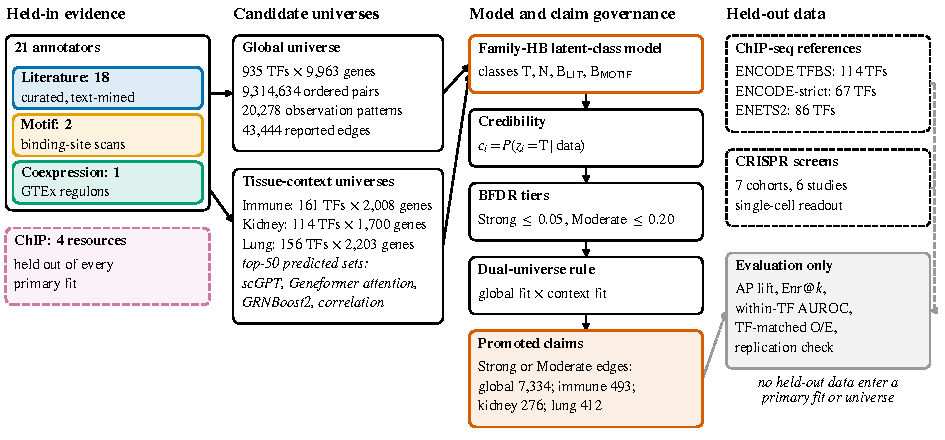
\includegraphics[width=\textwidth]{fig1_design.pdf}
  \caption{\textbf{Study design.} 21 held-in annotators in three evidence families (literature 18, motif 2, coexpression 1) report TF--target edges; the ChIP family (4 resources) is held out of every primary fit. The global universe contains 935 literature-covered TFs $\times$ 9{,}963 genes (9{,}314{,}634 ordered pairs, 20{,}278 distinct observation patterns, 43{,}444 edges with at least one report); the tissue-context universes contain the pairs both foundation models can score (immune 323{,}127, kidney 193{,}686, lung 343{,}512 pairs), in which scGPT and Geneformer attention, GRNBoost2 and correlation define predicted sets (top 50 targets per TF). Family-HB assigns every edge a credibility; BFDR tiers (Strong: BFDR $\leq 0.05$; Moderate: $\leq 0.20$) and, in the tissue universes, the dual-universe rule turn credibilities into graded claims; Strong and Moderate edges are promoted (global 7{,}334; immune 493, kidney 276, lung 412). Held-out ChIP-seq references (ENCODE TFBS, 114 TFs; ENCODE-strict, 67; ENETS2, 86) and 7 CRISPR perturbation cohorts from 6 studies enter no primary fit, universe definition or choice of the primary analysis (dashed: evaluation only); the tuning-optimism analysis uses perturbation labels only to measure what tuning on them would gain, and nothing it selects is used elsewhere.}
  \label{fig:design}
\end{figure}

